\documentclass{beamer}

\usetheme{Hokie}
\usepackage{palatino}
\usepackage{amsmath}

\title{Graph Algorithms for  Visualizing High Dimensional Data}
\author{Abhinav Shankaranarayanan Venkataraman}
\institute{Universitat Politecnica de Catalunya (UPC), Barcelona}
\date{27 June 2016}

\graphicspath{{./}}
\DeclareGraphicsExtensions{.png}
\logo{
\includegraphics[height=0.5cm]{logo.png}}
\setbeamertemplate*{logo}
\newcommand{\HRule}{\rule{\linewidth}{0.5mm}} % Defines a new command for the horizontal
\begin{document}

\frame{\titlepage}

\section[Outline]{Outline}
\frame{\tableofcontents}
\section{Project Details}
\frame{
\frametitle{Project Research Group}
The project is done under the umbrella of LARCA(Laboratory
for Relational Algorithmics, Complexity and Learning)
  Project Directors :
  \begin{itemize}
  \item Prof. Ricard Gavalda Mestre
    \item Prof. Marta Arias Vicente
  \end{itemize}
}
\section{Introduction}
\subsection[What is a Community?]{Community Structure}
\frame{
\frametitle{What is Community?}
				\begin{figure}
	\centering
	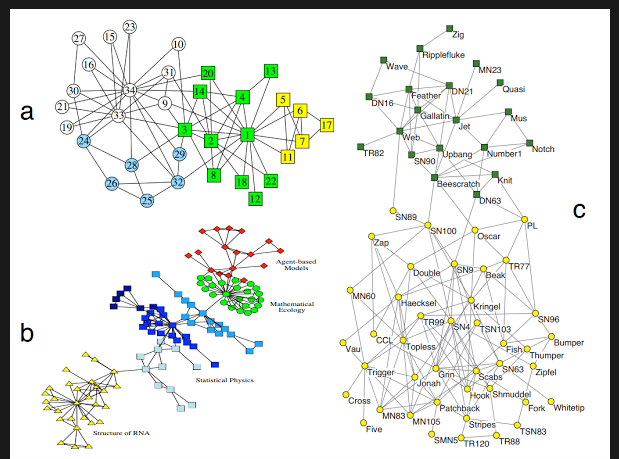
\includegraphics[scale=0.3]{comm.png}
	\caption{Communities: \cite{communitypaper}}
	\label{fig:test_down_sampling}
	\end{figure}

}
\subsection{Goal of the Project}
\frame
{
	\frametitle{Goal of the Project}
	\begin{enumerate}
\item To survey a few algorithms that aim in community finding keeping in mind that the input is from the medical domain. 
\item To choose an algorithms that benefit the purpose of organizing graphs from medical domain and for the purpose of visualization.
\item To implement the algorithms and test the efficiency of the algorithm using variety of graphs.
\item To build a Graphic User Interface (GUI) which enables visualization of the raw input on a web browser by drawing graphs.

\end{enumerate}
}
\subsection{Planning}

\frame{
\frametitle{Planning}
Planning is one of the most important part of any project. In this project we divide the project into five planning phases or stages namely,
\begin{itemize}
\item Required knowledge acquisition

\item Paper Analysis

\item Design and Implementation
\item Testing I
\item Testing II

\item Report Writing

\end{itemize} 

}

\subsection{Economic Budget}
\frame{
\frametitle{Economic Budget}
We divide the budget into 3 major categories:
\begin{itemize}
\item Hardware  budget
\item Software Budget
\item Human Resource Budget

\end{itemize} 
Total budget is the sum total of the three budget.
\\
\textbf{Amortized cost} : Amortized cost is that accumulated portion of the recorded cost of a fixed asset that has been charged to expense through either depreciation or amortization.
}

\subsection{Sustainability}
\frame
{
\frametitle{Sustainability}
The project is 
\begin{itemize}
\item Economically sustainable
\item Socially sustainable
\item Environmentally sustainable
\end{itemize}
}
\section{Background}

\subsection[Few Theoretical Concepts]{Graphs}

\frame
{
	\frametitle{Graph}
	A Graph $G$ is formed by two finite sets, the set \textit{V} = \{ $v_1,v_2, \ldots ,v_n$ \} of vertices(also called nodes) and the set \textit{E} = \{ $e_1,e_2, \ldots,e_n$  \} of edges where each edge is a pair of vertices from \textit{V}, for instance,
\begin{center}
$e_i = (v_j,v_k)$
\end{center}
is an edge from $v_j$ to $v_k$ represented as \textit{G}=(\textit{V},\textit{E}).
}


\section{Louvain Community Detection Algorithm}

\frame
{
	\frametitle{Louvain Community detection Algorithm}

	This section has some examples of common slideshow elements.
}

\subsection{Introduction to Louvain}

\frame
{
	
}




\section{Conclusions}
\subsection{Personal Learning}


\subsection{Personal Learning}

\frame
{
	\frametitle{Personal Learning}
Since the project had more scope for exploration.
My interest in Data Visualization has increased.
My interest in graphs has increased.
My python programming skill has also increased along with that I have also learned to code for web technologies on my own.
}

\subsection{Softwares and tool kits that were used}

\frame
{
	\frametitle{Software tools}
	\begin{enumerate}
		\item git
		\item github pages
		\item Linux OS
	\end{enumerate}
}


\section{About}
\subsection{Last Slide}

\frame
{
	\frametitle{About}

	This slide show is mostly to demo the Hokie Beamer theme and see how it looks in various slideshow elements.  Some parts of the presentation are taken from Jean-Etienne Poirrier's example presentation, which can be found here:  \href{http://www.poirrier.be/~jean-etienne}{http://www.poirrier.be/~jean-etienne}.
	
	
\bibliographystyle{plain}
\bibliography{mybib}{}
}

\section{References}

\frame
{
	\frametitle{List of References that were used}

\bibliographystyle{plain}
\bibliography{mybib}{}
}
\section{Gracies}

\frame
{
	\frametitle{Thank you}
Thank you for all those who supported me throughout the project.\\
It was a Great time at Barcelona working with Prof.Ricard and Prof.Marta.
\bibliographystyle{plain}
\bibliography{mybib}{}
}

\end{document}
